\section{Week 11 : DHT(s)}
\subsection{Introduction to Distributed Hash Tables (DHTs)}

A Distributed Hash Table (DHT) is a decentralized distributed system that provides a lookup service similar to a hash table; (key, value) pairs are stored in a DHT, and any participating node can efficiently retrieve the value associated with a given key. Responsibility for maintaining the mapping from keys to values is distributed among the nodes, in such a way that a change in the set of participants causes a minimal amount of disruption. This allows a DHT to scale to extremely large numbers of nodes and to handle continual node arrivals, departures, and failures.

DHTs are a fundamental building block for many distributed systems. They form the basis of many peer-to-peer (P2P) applications, distributed file systems, and databases.

\subsection{Table ADT}

A table, as an Abstract Data Type (ADT), is a fundamental concept in computer science. It's a structure that stores key-value pairs and supports, at a minimum, the following operations:

\begin{enumerate}[itemsep=1pt, topsep=1pt]
    \item \texttt{add(key, value)}: Inserts a new key-value pair into the table.
    \item \texttt{get(key)}: Retrieves the value associated with a given key.
\end{enumerate}

This seemingly simple structure allows for great flexibility and, more importantly, hides implementation details from the user. The data could be stored on your local machine, in the cloud, or, in our current topic of discussion, distributed across nodes in a network.

\subsection{Basic Distributed Hash Table Implementation: A Linear Ring}

\subsubsection{Concept}

The simplest way to visualize a DHT is as called \textbf{Chord} which is essentially a ring.  Imagine all possible keys (which we'll assume are integers for now) laid out in a circular fashion, from some minimum value (often $0$) to some maximum value (e.g., $2^n - 1$, where $n$ is the number of bits in the key).  Each node in the system is assigned a random ID within this key space. We will use a hash function to map data keys to this key space.

Each node is responsible for a segment of the key space.  Specifically, a node is responsible for all keys between its \textit{predecessor's ID} (exclusive) and its own \textit{ID} (inclusive).  This forms a \textit{keyspace}.

\begin{figure}[h]
\begin{center}
\begin{tikzpicture}[
  node/.style={rectangle, draw, fill=blue!20, minimum width=2cm, minimum height=1cm, align=center},
  arrow/.style={-Latex, thick}
]

\node[node] (0) at (-1, 2.8) {Bootstrap Node, id 0 \\ Successor: 45};
\node[node] (45) at (3.2, -1) {Node, id 45 \\ Successor: 99};
\node[node] (99) at (-1.8, -2.8) {Node, id 99 \\ Successor: 0};

\draw (0, 0) circle (3cm); % The circles

\draw[arrow] (0) -- (45);
\draw[arrow] (45) -- (99);
\draw[arrow] (99) -- (0);

\end{tikzpicture}
\end{center}
\label{fig:chord_ring}
\caption{Chord Ring Structure with Three Nodes}
\end{figure}

\subsubsection{Joining the Ring}
When a new node wants to join the ring, it does the following:

\begin{enumerate}[itemsep=1pt, topsep=1pt]
    \item \textbf{Bootstrap Node}: The new node contacts a known node in the ring.  This initial contact point is often called the \textit{bootstrap node}.  In the simplest case, the bootstrap node could initially hold all keys and values.

    \item \textbf{Key Range Calculation}: Upon connection, the new node announces a random ID chosen from within a specific key range. If the random key already exists in the network, leave the network and connect again with a new key. 

    \item \textbf{Insertion}: The new node is inserted into the ring, and the keyspace responsibilities are adjusted.  The new node becomes the \textit{successor} of its \textit{predecessor}, and the \textit{predecessor} of its \textit{successor}.
\end{enumerate}

\subsubsection{Lookup Operation}
The lookup operation is the core of a DHT. Here's how it works in this basic linear ring:

\begin{enumerate}[itemsep=1pt, topsep=1pt]
    \item \textbf{Start Query}: A node receives a query for a specific key.

    \item \textbf{Check Keyspace}: The node checks if the key falls within its own keyspace (between its predecessor's ID and its own ID).

    \item \textbf{Forward Query (if necessary)}:
    \begin{itemize}[itemsep=1pt, topsep=1pt]
        \item If the key is within the node's keyspace, the node returns the corresponding value.
        \item If the key is \textit{not} within the node's keyspace, the node forwards the query to its \textit{successor}.
    \end{itemize}

    \item \textbf{Iterative Process}: This process (check keyspace, forward if necessary) repeats until the node responsible for the key is found.
\end{enumerate}


\begin{minipage}{0.60\textwidth}
Initially, you may have node 0 as the bootstrap, which \texttt{owns} the entire key space.
Then, let's imagine nodes with IDs 3 and 10 join. The ring might look like the graph on the right:

In this case, we can view the connections between the nodes as a doubly linked list. This list represents the ring.

\begin{itemize}[itemsep=1pt, topsep=1pt]
    \item Node 3 is responsible for keys 1, 2, and 3.
    \item Node 10 is responsible for keys 4, 5, 6, 7, 8, 9, and 10.
    \item Node 0 is responsible for keys 0, 11, 12, 13, 14, and 15.
\end{itemize}	
\end{minipage}
\hfill
\begin{minipage}{0.3\textwidth}
\begin{center}
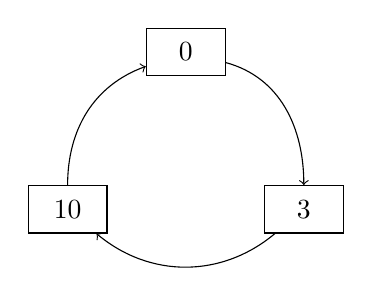
\begin{tikzpicture}
    % Nodes with rectangles
    \node[draw, rectangle, minimum width=1cm, minimum height=0.6cm] (zero) at (0,2) {0};
    \node[draw, rectangle, minimum width=1cm, minimum height=0.6cm] (three) at (1.5,0) {3};
    \node[draw, rectangle, minimum width=1cm, minimum height=0.6cm] (ten) at (-1.5,0) {10};

    % Edges with arrows
    \draw[->] (zero) to[out=-15, in=90] (three);
    \draw[->] (three) to[out=220, in=-40] (ten);
    \draw[->] (ten) to[out=90, in=200] (zero);
\end{tikzpicture}
\end{center}
\end{minipage}



\subsubsection{Leaving the Ring (Graceful Shutdown)}

If a node wants to leave the ring gracefully (i.e., not a sudden failure), it should:

\begin{enumerate}[itemsep=1pt, topsep=1pt]
    \item \textbf{Notify Successor}: The leaving node tells its \texttt{successor} that it has a new \texttt{predecessor} (the leaving node's predecessor).
    \item \textbf{Pointer Update}: The successor's \texttt{prev} pointer should be updated to the same value that was in the exiting node's \texttt{prev} pointer.
\end{enumerate}


\subsection{Handling Node Failure}

\subsubsection{The Problem}

In a distributed system, nodes can fail (e.g., crash, lose network connectivity). If a node fails, queries that need to traverse that node will also fail.  In our simple linear ring, if the successor node is unreachable, there's no way to route around the failure.

\subsubsection{Detection}

How do we detect that a node has failed?  One approach is to have nodes periodically send \texttt{ ping} messages to their successors.  If a node doesn't receive an \texttt{acknowledgment (ACK)} message back within a certain timeout period, it assumes its successor has failed.

\subsubsection{Recovery (Basic)}

If a node detects that its successor has failed, it can:

\begin{enumerate}[itemsep=1pt, topsep=1pt]
    \item \textbf{Query the Bootstrap}:  The node contacts the bootstrap node (or any other known node in the ring).
    \item \textbf{Rejoin the Ring}:  The node essentially rejoins the ring as if it were a new node. It contacts another node in the ring to insert itself, taking over the keyspace of the failed node.
\end{enumerate}

\subsection{Improving Lookup Performance: Finger Tables}

\subsubsection{The Problem with Linear Lookup}

With a simple linear ring, lookup time is $O(n)$, where $n$ is the number of nodes.  This is because, in the worst case, a query might need to traverse the entire ring.  This is unacceptably slow for a large distributed system.

\subsubsection{The Solution: Finger Tables}

To speed up lookups, each node maintains a \textit{finger table}.  The finger table is a set of pointers (or indexes) to other nodes in the ring, spaced at exponentially increasing distances.

The $i^{th}$ entry in the finger table of node \textbf{n} points to the first node that succeeds $n + 2^i \pmod{2^n}$.

So, a node with ID 0 would have a finger table containing:
\begin{itemize}[itemsep=1pt, topsep=1pt]
    \item id + $2^0$
    \item id + $2^1$
    \item id + $2^2$
    \item id + $2^3$
    \item ...
    \item id + $2^{n-1}$
\end{itemize}
And each successive entry would store a node that is at least that far away from it in the ring.

\begin{example}{Example Finger Table for 8 nodes}
\makebox[\textwidth][l]{ % Ensures both minipages are properly aligned
    \begin{minipage}{0.6\textwidth}
        In Table~\ref{tab:finger_table}:
        \begin{itemize}[itemsep=1pt, topsep=1pt]
            \item The ID is implicit (the node for which this is a table).
            \item id + $2^i$ is the target key.
            \item "successor" is the ID of the node responsible for that target key (or the next closest node in the ring).
        \end{itemize}	
    The advantage of a finger table is that it enables logarithmic lookup. With each hop, the distance to the destination key is roughly halved.
    \end{minipage}
    \hfill
    \begin{minipage}{0.35\textwidth}
        \centering
        \begin{tabular}{|c|c|c|}
            \hline
            $i$ & id + $2^i$ & successor \\ 
            \hline
            0 & 1  & 3  \\
            1 & 2  & 3  \\
            2 & 4  & 6  \\
            3 & 8  & 10 \\
            \hline
        \end{tabular}
        \captionof{table}{Finger Table}
        \label{Finger-table}
    \end{minipage}
}
\end{example}


\subsection{Race Conditions and Connection Issues}

\subsubsection{Race Conditions}

Because nodes can join and leave concurrently, race conditions can occur. For example, two nodes might try to become the successor of the same node simultaneously.  The Chord protocol uses the "last writer wins" rule (using timestamps or some other ordering mechanism) to resolve these conflicts.

\subsubsection{Connection Issues}

Nodes might be temporarily unreachable due to network problems. The system needs to be robust to this.  Periodic checks (pings) and retries are essential.  UDP is typically used for communication due to its connectionless nature, allowing messages to be sent and received without maintaining a persistent connection.  However, this also means UDP is unreliable, and messages might be lost.

\subsection{Further Considerations}
\begin{itemize}[itemsep=1pt, topsep=1pt]
\item \textbf{Consistency Models}: Distributed systems often use \textit{eventual consistency}, meaning that updates will eventually propagate through the system, but there might be temporary inconsistencies.

\item \textbf{Fault Tolerance}:  DHTs are designed to be fault-tolerant.  The failure of a single node should not bring down the entire system. Data replication is commonly used to further enhance fault tolerance.

\item \textbf{Security}:  In real-world deployments, DHTs need to consider security aspects.  How do you prevent malicious nodes from joining the ring and disrupting lookups or corrupting data?

\item \textbf{Chord and Other DHT Algorithms}: Chord is a specific, well-known DHT algorithm. Other algorithms like Kademlia, Pastry, and Tapestry exist, each with different trade-offs in terms of performance, complexity, and robustness.

\item \textbf{Real-World Applications}: DHTs are used in BitTorrent (for tracking peers), distributed databases (like Cassandra and Riak), and many other distributed systems.
\end{itemize}


\endclass{Week 11}
